\section{Measuring and Predicting the Performance of Highly Configurable Systems}\label{sec:measuring}

By learning about the performance difference of multiple configurations it is possible to predict a program's performance accurately. This means, that not all (possibly exponentially many) configurations need to be measured. Instead, a small sample size should be enough to predict a program's performance. Multiple ways that use different methods have been proposed over time \cite{FasterDiscoveryofFasterSystemConfigurationsSiegmund2017}. This paper will take a look at
\begin{itemize}
	\item \hyperref[sec:AFID]{Automated Feature Interaction Detection} by \citet{AutomatedFeatureDetectionSiegmund2012},
	\item an \hyperref[sec:VAPP]{incremental/statistical learning approach} by \citet{VariabilityAwarePerformancePredictionJianmeiSigmundApel},
	\item \hyperref[sec:CESampling]{Cost efficient sampling by \citet{CostEfficientSampling_Gou_Siegmund_2015}},
	\item \hyperref[sec:WHAT]{\textbf{WHAT}} a spectral learning approach by \citet{FasterDiscoveryofFasterSystemConfigurationsSiegmund2017},
\end{itemize}

\subsection{General Approach}

\citet{VariabilityAwarePerformancePredictionJianmeiSigmundApel} defines two problems to be solved by prediction approaches:
\begin{enumerate}
	\item Predicting the performance of a not measured configurations.
	\item Finding a function $f$ that shows the correlation between the properties of measured configurations and their performance value and that makes each predicted performance $f(\x)$ of a configuration $\x$ as close as possible to its actual performance.\\	
	\begin{equation}
	f : \mathcal{C} \rightarrow  \mathbb{R} \text{ such that} \sum_{(\x,y) \in S} L(y,f(\x)) \text{ is minimal}
	\end{equation}\\
	$S$ is a sample and	$L$ is a loss function to penalize errors in prediction. $(\x,y)$ is a pair of a configuration and its measured performance value. The function $f$ is sometimes called the \textit{performance model} of the system.
\end{enumerate}

\noindent
There is a general pattern for the solution of those problems that comes apparent when looking at different prediction approaches. It can be divided into two steps as displayed in \cref{fig:GeneralApproach}.\begin{figure}
	\includegraphics[page=9,clip,trim=4.1cm 5.9cm 3.9cm 19.4cm, width=\textwidth]{presentation/presentation}
	\caption{General pattern of prediction approaches. }
	\label{fig:GeneralApproach}
\end{figure}

The first step is to sample the exponential configuration space. This means finding configurations from which can be learned about the system. This is done by using efficient sampling techniques like spectral sampling \cite{DistanceBasedSampling2019} or progressive sampling \cite{CostEfficientSampling_Gou_Siegmund_2015}.

Once enough and meaningful configurations are found, the learning process starts. Usually the previously chosen configurations are measured, under the condition that this was not already done whilst sampling. The measurement results are fed to a learning process. A lot of different machine learning strategies can be applied \cite{VAMOSConference}. The relative papers typically use \CART's. Based on the found performance model continuing tasks like finding near optimal solutions or in-depth performance analysis can be done \cite{VAMOSConference}.


%\subsection{Approaches to Performance Prediction}\label{sec:approachesPerformanceLearning}

Before looking at actual prediction methods one should have a look at general possibilities for prediction methods. There are 2 general approaches to predicting a component-based system's performance \cite{ComparativeanalysisAbdelaziz112011}. 

\subsubsection[Measurement Approach]{\textnormal{First there is the }measurement-based approach\textnormal{.}} A measurement-based approach uses an analysis tool to monitor an application during execution. Based on the measurements of an existing application a performance model is build and modified. This approach is highly dependent on existing software (e.g.: measured application, analysis tool, operating system). \cite{ComparativeanalysisAbdelaziz112011}

\subsubsection[Model-based Approach]{\textnormal{Secondly there is the }model-based approach\textnormal{.}}
A model-based approach relies on models created by Model Driven Development. It combines multiple models of a system to give a performance prediction. The advantage of this technique is that it does not require a system to exists. Therefore performance modelling can be done before a system is actually composed.
Automation and usage profiles are used to improve the prediction accuracy of this method. Approaches that don't use automation are generally found to be reasoning tools rather than applicable approaches. Some approaches do not consider external factors such as external service calls, usage profiles or the execution environment at all. This decreases the accuracy of their predictions. \cite{ComparativeanalysisAbdelaziz112011}

\subsubsection[Mixed Approaches]{Mixed approaches} are also possible and can occur in many different variations. For example it is possible to parametrize a model based on measured values. \cite{ComparativeanalysisAbdelaziz112011}

This paper will mainly focus on measurement based approaches.%TODO reasoning

%\citet{ComparativeanalysisAbdelaziz112011} also provide an overview over the benefits and disadvantages of each type of approach:





\subsection{Automated Feature Interaction Detection}\label{sec:AFID}

Automated feature interaction detection (AFID) is a measurement-based approach to predicting the performance of a highly configurable system.
It was developed by \citet{AutomatedFeatureDetectionSiegmund2012}. Unlike other methods it does not depend on machine learning but rather tires to directly identify the performance impact of each feature or a combination of features. This method reached a precision of up to 95\% in the experiment conducted by  \citet{AutomatedFeatureDetectionSiegmund2012}.

\subsubsection[Formulars]{\textnormal{Some} Formulars} are needed to descibe a Softwaresystem for AFID .
The composition of using two (or more) units/features is denoted by $\cdot$ . This composition is also called a configuration \cite{VariabilityAwarePerformancePredictionJianmeiSigmundApel}.\\
The interaction of two features is denoted by $a\#b$. By combining both we get a feature interaction:
\begin{equation}
 a \times b = a\#b \cdot a \cdot b
\end{equation} 
This equation expresses, that when using both $a$ and $b$ we also need to consider their interaction $a\# b$. Note that either $a$ or $b$ can also be a configuration.\\
Further Sigmund uses an abstract performance function $\Pi$ that is used to represent some performance value of a configuration:
\begin{align}
\Pi(a \cdot b) &= \Pi(a) + \Pi(b)\label{eq:featureInteraction_SimplePerformance}\\
\Pi(a\#b) &= \Pi(a \times b) - (\Pi(a) + \Pi(b))\\
\Pi(a \times b) &=  \Pi(a\#b) + (\Pi(a) + \Pi(b))\label{eq:featureInteraction_InteractionPerformances}
\end{align}
Following that the performance of a program $P = a \times b \times c$ can be written down as
\begin{equation}\label{eq:featureInteraction_ProgrammPerformance}
\Pi(P) = \Pi(a) +  \Pi(b) +  \Pi(c) +  \Pi(a\#b) +  \Pi(a\#c) +  \Pi(b\#c) +  \Pi(a\#b\#c). 
\end{equation}
The Problem with the equations \ref{eq:featureInteraction_SimplePerformance}-\ref{eq:featureInteraction_ProgrammPerformance} is that they assumes that we can measure the performance of a feature in isolation. This is in general not possible \cite{AutomatedFeatureDetectionSiegmund2012}. Also we are still in the space of $\mathcal{O}(2^n)$ of possible configurations that we need to measure.  
To reduce this Sigmund et al. uses a interaction \textit{delta}. 
\begin{equation}
\begin{split}
\Delta a_C &= \Pi(C\times a) - \Pi(C)\\
&=\Pi(a\# C) + \Pi(a)
\end{split}
\end{equation}
Where $C$ is a base configuration. This formula describes how the performance influence ($\Delta$) of $a$ on a configuration $C$ can be calculated. Its either the performance difference between using $C$ with and without $a$, or the performance influence of $a$ itself plus the influence of the interaction between $C$ and $a$.\\
As a general approach to reduce its search space AFID looks at:\\
\begin{minipage}{\textwidth}
\begin{equation}
	\Delta a_{min} = \Pi(a \times min(a)) - \Pi(min(a))
\end{equation}
\begin{center}
	and
\end{center}
\begin{equation}
	\Delta a_{max} = \Pi(a \times max(a)) - \Pi(max(a))
\end{equation}
\end{minipage}\\[0.3cm]
 Where $min(a)$ is a valid minimal configuration not containing $a$ but to which $a$ can be added to create another valid configuration. $max(a)$ is a valid maximal configuration not containing $a$ but to which $a$ can be added to create another valid configuration.\\
 \subsubsection[Automated Feature Interaction Detection]{\textnormal{For} AFID} 
one first needs to define when a feature is interacting. For this \citet{AutomatedFeatureDetectionSiegmund2012} use the definition of 
 \begin{equation}
 a \text{ interacts} \Leftrightarrow \exists C,D | C \neq D  \land	 \Delta a_C \neq \Delta a_D .
 \end{equation}
 $C~=~min(a)$ and $D~=~max(a)$ are chosen to find interacting features and to reduce the search space for $C$ or $D$ from $\mathcal{O}(2^n)$ to $\mathcal{O}(n)$. By measuring $\Delta a_{min(a)}=\Delta a_C$ and $\Delta a_{max(a)}=\Delta a_D$ for each feature some first information about their behavior can be obtained. If both values for a feature $a$ are similar it does not interact with the features of $max(a)\backslash min(a)$. Otherwise $a$ is marked as interacting. In both cases it can still interact with the features of $min(a)$. In total 4 measurements per feature are required ($\Pi(a \times min(a))$, $\Pi(min(a))$, $\Pi(a\times max(a))$, $\Pi(max(a))$)\cite{AutomatedFeatureDetectionSiegmund2012}.\\
 Since most of the interacting features are known by now one can look for the groups of features whose interaction does have an influence on performance. Again the problem arises that there is an exponential number of possible combinations. Three heuristics are used to simplify the finding of these groups.
 
 \newcommand{\oitem}[2]{{\item[{\parbox[t][0pt][t]{\leftmargin}{\raggedleft #1}}] {\parbox[t]{\textwidth-\leftmargin}{#2}}}}
 \begin{itemize}[leftmargin=4cm]
 	\setlength\itemsep{1em}
 	\oitem{Pair-Wise~Heuristik (PW):\label{lab:PW}}{ Most groups of interacting features appear in the size of two\cite{AutomatedFeatureDetectionSiegmund2012,AnalysisOfTheVariabilityInFortyPreprocessor_BasedSPLLiebig}. So it makes sense to look for pair interaction first.}
 	\oitem{Higher-Order Interactions Heuristic (HO):\label{lab:HO}}{
 		\citet{AutomatedFeatureDetectionSiegmund2012} only look at higher order interactions of the rank of three. More on this later.
 	}
 	\oitem{Hot-Spot Features (HS):\label{lab:HS}}{
 		Based on \cite{FeatureCohesioninSPL, CanWeAvoidHighCoupling?} \citet{AutomatedFeatureDetectionSiegmund2012} assume that hot spot features exist. \inlineQuote{[...] There are usually a few features that interact with	many features and there are many features that interact only with few features.}, these features are the hot spot features.
 	}
 \end{itemize}
Using a SAT-Solver an implication graph as seen in \autoref{fig:ImplicationTree} is generated. Each implication chain in this tree should have at least one interacting feature. When analysing the tree each chain is walked from the top down. The three heuristics will be applied in the order of PW $\rightarrow$ HO $\rightarrow$HS.  

\begin{wrapfigure}{l}{0.5\textwidth}
%\setlength\belowcaptionskip{-\baselineskip}
\includesvg[width = 0.5\textwidth]{figures/ImplicationTree}
\captionsetup{width=0.95\linewidth}
\caption{Implication tree example found in \cite{AutomatedFeatureDetectionSiegmund2012} }
\label{fig:ImplicationTree}
\end{wrapfigure}

First the influence of every feature on another chain is measured (\hyperref[lab:PW]{PW-heuristic}). In the example of \autoref{fig:ImplicationTree} the interactions would be measured in this order:\inlineQuote{$F1\#F6, F1\#F7, F4\#F6,\\ F4\#F7, F6\#F11,F7\#F11,F1\#F11,\\ F4\#F11$}\cite{AutomatedFeatureDetectionSiegmund2012}. If an interaction impact $\Delta a\#b_C$ exceeds a threshold it is recorded.

Secondly, the \hyperref[lab:HO]{higher order interaction heuristic} is applied. Higher order interactions can be relatively easily found by looking hat the results of the PW-Heuristik. Three features that interact pair-wise are likely to interact in a third order interaction. For example, looking at features $a$, $b$ and $c$- If $\Delta a\#b_{C1}$ and $\Delta b\#c_{C2}$ have been recorded $\{a\#b, b\#c, a\#c\}$ all have to be non zero to find a third order interaction. Interactions with and order higher than three are not considered to prevent too many measurements.

Lastly Hot-Spot features are detected (\hyperref[lab:HS]{HS-heuristic}). This is done by counting the interactions per feature. If the number of interactions of a feature is above a certain threshold (e.g. the arithmetic mean) it is categorized as a Hot-Spot feature. Based on the hotspot features further third order interactions are explored. Again higher order interactions are not considered to prevent too many measurements. \\
After applying the three heuristics all detected interacting features or feature combinations are assigned a $\Delta$ to represent their performance influence on the program.

\begin{wrapfigure}{r}{.5\textwidth}
	\centering
	\setlength\belowcaptionskip{-2\baselineskip}
	\captionof{table}{Results of average accurcy found by \citet{AutomatedFeatureDetectionSiegmund2012}}
	\label{tab:avgAccuracy}
	\begin{tabular}{c|c}
		Approach&avg. Accuracy\\\midrule[1pt]
		FW&79.7\%\\\hline
		PW&91\%\\\hline
		HO&93.7\%\\\hline
		HS&95.4\%\\\hline
	\end{tabular}
\end{wrapfigure}\noindent
\citet{AutomatedFeatureDetectionSiegmund2012} tested AFID on six different SPLs (Berkely DB C,Berkely DB Java, Apache, SQLite, LLVM, x264). Each program was tested under four approaches: Feature-Wise, Pair-Wise, Higher-Order, Hot-Spot (in this order). Each approach also used the data found by the previous one. Accordingly the results get better the more heuristics are used as seen in \cref{tab:avgAccuracy}. Using only the FW approach means that interactions (and the heuristics) are not considered, yet the accuracy is already at about 80\% on average. A significant improvement can be made by using the PW heuristic. It uses on average 8.5 times more measurements than the FW approach but improves the accuracy to 91\%. Using the HO or HS approach improves the accuracy further by about 2-4\%. However for Apache using the HO over the PW approach even deteriorated the average result by 3.9\% and doubled the standard variation. As already mentioned using the HS approach gives the best accuracy this is true for all 6 tested applications. \citet{AutomatedFeatureDetectionSiegmund2012} also notes that analysing SQLite only needed about 0.1\% of all possible configurations. This hints to the good scalability of AFID.

\subsection{Classification and Regression Trees}
\label{sec:CART}
The next 3 approaches all use a specific type of machine learning strategy to construct their predictors. This method is call Classification and Regression Tree's (\CART). These trees are typically binary trees that divide the given data points into small enough groups so a direct local prediction can be done.
These local prediction are than combined into a global predictor \cite{VariabilityAwarePerformancePredictionJianmeiSigmundApel}. In the context of configurable software systems each point consists at least out of a configuration and an associated performance score. These data point are then fed into the algorithm seen in \cref{alg:CART}.
\begin{figure}[h]
	\lstset{
		mathescape,
		breaklines=true,
	}
	\begin{lstlisting}
1. Start at the root node. Assign all configurations to it.
2. For each option, find the set of options $X$ that minizes the sum of the node impurities in the two child nodes. Divide the configurations assigned to the current node based on $X$ into two disjoint sets and assign those to the corresponding child nodes.
3. If a stopping criterion is reached, exit. Otherwise, apply step 2 and 3 to each child node inturn.
	\end{lstlisting}
	\captionof{lstlisting}{Pseudocode for generating a \CART. Adopted from \citet{ClassificationAndRegressionTrees} to fit software configurations.}
	\label{alg:CART}
\end{figure}
The node impurity is typically calculated by the square mean error. As a stopping criteria the size of the leaf node is used \cite{VariabilityAwarePerformancePredictionJianmeiSigmundApel}. The size of the predictor variables set $X$ is usually 1.
\begin{figure}[h]
	\centering
	\includegraphics[page=4,clip,trim=3.5cm 18cm 3.5cm 1.5cm, width=\linewidth]
	{Paper/VariabilityAwarePerformancePredictionAStatisticalLearningApproach.pdf}
	\caption{Example performance model of X264 generated by CART based on the random sampling, using minimization of the sum of squared error loss \cite{VariabilityAwarePerformancePredictionJianmeiSigmundApel}.}	
	\label{fig:VAPPExampleTree}	
\end{figure}


\subsection{Variability aware Performance Prediction}\label{sec:VAPP}

Variability aware Performance Prediction (\VAPP) is a statistics based approach to performance prediction. With the help of random sampling and \CART s a simple yet effective predictor can be build. The following section is based upon \citet{VariabilityAwarePerformancePredictionJianmeiSigmundApel}. In their own tests \citet{VariabilityAwarePerformancePredictionJianmeiSigmundApel} reached an average precision of 94\% whilst using a sample as large as the ones \AFID~would be using under the PW-heuristic. Further, tests conducted by \citet{FasterDiscoveryofFasterSystemConfigurationsSiegmund2017} with the same sample size showed an accuracy of 92.4\%.\\
\setlength\intextsep{\baselineskip}
\begin{wrapfigure}[12]{R}{.5\linewidth}
	\includegraphics[page=3,clip,trim=11cm 13.5cm 1.5cm 10.25cm, width=\linewidth ]{Paper/VariabilityAwarePerformancePredictionAStatisticalLearningApproach}
	\caption{Overview of the Approach of Variability aware Performance Prediction \cite{VariabilityAwarePerformancePredictionJianmeiSigmundApel}.}
	\label{fig:VAPPOverview}
\end{wrapfigure}
The basic idea of variability aware performance prediction is shown in \cref{fig:VAPPOverview}.
Two cycles can be found:	
\FloatBarrier 
\begin{itemize}	
	\item[$\circ$] The first cycle is outside of the dashed box and describes the basic input-output behavior of a predictor. A user configures a new configuration $\x$ for System $A$ and asks the predictor (dashed box) for a prediction. It replies with a quantitative prediction for $\x$'s performance.
	\item[$\circ$]  In the second cycle a actual prediction is generated based on decision rules which themselves are in turn created by simplifying a performance model (a \CART). Random sampling is used to learn the performance model.
\end{itemize}
Like other approaches, the target of variability aware performance prediction is to get accurate predictions whilst only using a small sample for the creation of the performance model. Nonetheless, \VAPP~offers a free choice of the sample size. The configurations of the sample are chosen randomly out of $\mathcal{C}$. 

\VAPP~uses the tuple-based definition of a configuration. It further defines that each configuration $c_j \in \mathcal{C}$ has an actual performance value $y_j$. For formal correctness it is assumed that every option of a configuration actually influences the performance of the system. Otherwise, a \CART~could not be applied.

In the used \CART~each sub-tree is also called a segment $S_i$, where $i$ determines the location of the sub-tree. This is also shown in \cref{fig:VAPPExampleTree}.\\
For the \textit{local model} $\ell$ of the used \CART~\citet{VariabilityAwarePerformancePredictionJianmeiSigmundApel} choose the arithmetic average:
\begin{equation}
	\ell_{S_i} = \frac{1}{|S_i|} \sum_{y_j \in S_i} y_j
\end{equation}
As a loss function to penalize the prediction errors (node impurity) the sum of squared error loss is selected.
\begin{equation}
	\sum_{y_j \in S_i} L(y_j,\ell_{S_i}) = \sum_{y_j \in S_i} (y_j - \ell_{S_i})^2
\end{equation}
Therefore the best split for a segment $S_i$ is found when
\begin{equation*}
\sum_{y_j \in S_{iL}} L(y_j,\ell_{S_{iL}}) + \sum_{y_j \in S_{iR}} L(y_i,\ell_{S_{iR}})
\end{equation*}
is minimal.

Assuming there are $q$ leafs in a tree than the predictor function $f(\mathrm{x})$ is defined as:
\begin{equation}\textsl{}
f(\mathrm{x})=\sum_{i=1}^{q} \ell_{S_i}I(\mathrm{x}\in S_i)
\end{equation}
where $I$ is an indicator function to indicate whether $\mathrm{x}$ belongs to a leaf $S_i$.\\
For the example of \cref{fig:VAPPExampleTree}, $f(\mathrm{x})$ unwraps to:
\begin{align*}
f(x) = 255&* I(x_{14}=1,x_7=0)\\[-0.1cm]
	 + 268&* I(x_{14}=1,x_7=1)\\[-0.1cm]
	 + 402&* I(x_{14}=0,x_{15}=1,x_3=0)\\[-0.1cm]
	 + 508&* I(x_{14}=0,x_{15}=1,x_3=1)\\[-0.1cm]
	 + 571&* I(x_{14}=0,x_{15}=0,x_3=1)\\[-0.1cm]
	 + 626&* I(x_{14}=0,x_{15}=0,x_3=0)
\end{align*}
Every possible configuration $\mathrm{x}$ is associated with a leaf of the tree. Therefore, $f(\mathrm{x})$ can always be applied.\\

For their Experiment \citet{VariabilityAwarePerformancePredictionJianmeiSigmundApel} test the same software systems as \citet{AutomatedFeatureDetectionSiegmund2012} (\cref{sec:AFID}). They also compared their prediction results with the results produced by \AFID.\\
Since unlike \AFID~the size of a sample for \VAPP~can be chosen freely, some comparable sample sizes were chosen. \citet{VariabilityAwarePerformancePredictionJianmeiSigmundApel} use 4 different sample sizes based on the size of the tested programs. For a program with $N$ features they use samples the size of $N,2N,3N \text{ and } M$. $M$ is the amount of configurations measured by \AFID~using the \hyperref[lab:PW]{PW-heuristic}.
It was found, that the prediction accuracy increases linear with the size of a sample. For a small sample with the size of $N$ the prediction accuracy was at above 92\% in 3 cases. However, for Berkeley DB (C) the prediction accuracy with an $N$ sized samples was at 112.4\% with a standard deviation of $\pm$354.6\%. This shows that \VAPP~is not generally applicable for small samples.
Using a sample size of $M$ significantly improves the average prediction accuracy to a stable average of 93.8\%.\\

\subsection{Cost-Efficient Sampling}\label{sec:CESampling}
Just how its name suggests, cost-efficient sampling tires to minimize the cost-accuracy rate of a prediction approach. This is done by trying to find a (near) optimal sample size $n^*$ for a given program.\\
\citet{CostEfficientSampling_Gou_Siegmund_2015} apply two different sampling techniques to reach this goal. Their general structure is displayed in \cref{fig:CEGeneral}.
\newpage
\begin{figure}[h]
	\centering
	\includesvg[scale=.8,inkscapelatex=false]{figures/CEGeneral}
 	\caption{General procedure of cost-efficient sampling to find an optimal sized $n^*$.}
 	\label{fig:CEGeneral}
\end{figure}
\begin{wrapfigure}[21]{R}{.45\textwidth}	
	\includegraphics[page=2,clip,trim=12.8cm 16cm 3cm 6.2cm, width=\linewidth]{"Paper/Cost-Efficient Sampling for Performance Prediction of Configurable Systems".pdf}
	\captionsetup{width=0.9\linewidth}
	%\setlength\belowcaptionskip{2\baselineskip}
	\captionof{figure}{ A typical learnig curve can be divided into three phases:\\1. steep incline;\\2. gradual incline;\\3. plateau \cite{CostEfficientSampling_Gou_Siegmund_2015}.}
	\label{fig:learningcurve}
\end{wrapfigure}
Firstly a test and a training set are picked from $\mathcal{C}$. Then, in each iteration of this process, a performance model is build. The used sample is taken from the training set and is increased each iteration. This makes the respective performance model more accurate in each iteration. The error rate of each created performance model is recorded. Together with the size of the used sample a point in a graph is created. As iterations continue this graph resembles an approximation of the learning curve of the performance model of the system. A curve as displayed in \cref{fig:learningcurve} is created. This process continues until  a stopping criterion is met. At this point $n^*$ was already found or can be calculated based on the given curve and a cost-function. An optimal sample size should provide a good accuracy without being too large. Naturally $n^*$ lies somewhere at the beginning of the third phase.\\
Four different types of costs are considered by \citet{CostEfficientSampling_Gou_Siegmund_2015}:
\begin{equation}
\begin{split}
TotalCost &= Cost_{Measuerment(Training)}\\
&+ Cost_{Measuerment(Testing)}\\
&+ Cost_{ModelBuilding}\\
&+ Cost_{PredictionError}\\
\end{split}
\end{equation}

Based on this, the $TotalCost$ for a sample the size of $n$ is defined as:
\begin{equation}
TotalCost(n) = 2n + \epsilon_n \cdot |S| \cdot R \label{eq:costfunction}
\end{equation}

$S$ is a \textit{score set} that contains all configurations, whose performance value will be predicted with the current model. $R$ is tuning parameter for the measuring cost of a training set.

The two sampling strategies based on this are \textit{progressive sampling} and \textit{projective sampling}. Both approach the search for $n^*$ differently.

\setlength\intextsep{0pt}
\subsubsection{Progressive sampling}
\begin{wrapfigure}[28]{l}{.4\linewidth}
	\includegraphics[page=4,clip,trim=3.7cm 16.3cm 13.0cm 1.8cm, width=\linewidth]{"Paper/Cost-Efficient Sampling for Performance Prediction of Configurable Systems".pdf}
	\caption{Stopping criteria of \textit{progressive sampling}
	\cite{CostEfficientSampling_Gou_Siegmund_2015}.}
	\label{fig:progessiveSamplingStopping}
\end{wrapfigure}
can be divided into two different strategy types. They differ in the way the next sample size $n_{i+1}$ is calculated:
\begin{enumerate}
	\item arithmetic: $n_i= n_0 +i \cdot a$
	\item $\;$geometric: $n_i = n_0 + a^i$
\end{enumerate}
The constant parameter $a$ determines the growth-rate of the samples. On one hand arithmetic progressive-sampling is more precise, but on the other hand we need to build more performance models in comparison to geometric progressive-sampling.
For \textit{progressive sampling} there are two types of stopping criteria:
\begin{enumerate}
	\item Gradient-Based: Additional models around $n_i$ will be build so the gradient around at $n_i$ can be determined. \cref{fig:progessiveSamplingStopping}a shows an example of this. Once the gradient or accuracy reaches a certain threshold the iterative process is stopped and $n^*$ set as $n_i$.
	\item Cost Minimization: For each $n_i$ the current error-rate of the performance model is substituted into the cost function of \cref{eq:costfunction}. For well-behaved learning curves the cost function is convex as displayed in \cref{fig:progessiveSamplingStopping}b. Once the cost-function increases for the first time, the iterative process is stopped and $n^*$ set as $n_{i-1}$.
\end{enumerate}

\subsubsection{Projective sampling} tires to find the actual function behind the learning curve of the performance model of the current system. Typical equations that describe a learning curve and the respective minimum of the cost-function can be found in \cref{tab:learningCurveFunction}.
Unlike in \textit{progressive Sampling} the size of the sample set is increased by only a small amount each iteration. The experiments conducted by \citet{CostEfficientSampling_Gou_Siegmund_2015} show that even an increment by the size of 1 is enough to get satisfying results. This time the iterative process is stopped once a certain accuracy is reached. Now an algorithm tires to fit the generated points onto the four functions shown in \cref{tab:learningCurveFunction}. The best fitted function is considered the learning curve of the current performance model. Once this function is found, it can be substituted into to cost-function \cref{eq:costfunction} and the minimum of which can be calculated. These minimums are also shown in \cref{tab:learningCurveFunction}.
\setlength\intextsep{\baselineskip}
\begin{figure}[h]
	\centering
	\captionof{table}{Functional representation of typical learning curves and thier optimal sample size based on the given cost function \cite{CostEfficientSampling_Gou_Siegmund_2015}.}
	\label{tab:learningCurveFunction}
	\includegraphics[page=5,clip,trim=1.9cm 22.8cm 11.25cm 2.7cm, width=1\linewidth]{"Paper/Cost-Efficient Sampling for Performance Prediction of Configurable Systems".pdf}
\end{figure}
\noindent
Based on the found minimum other techniques that do not have a fixed sample size like \VAPP~can be used. In the experiments conducted by \citet{CostEfficientSampling_Gou_Siegmund_2015} \textit{projective sampling} was better than \textit{progressive sampling} in every case. For each of the six tested software systems \textit{projective sampling} had a better accuracy whilst having a lower cost than \textit{progressive sampling}.\\
For both strategies it is important, that the initial sample generation/picking is successful. Therefore, the picking of representative configurations as $n_i$ samples of each iteration is key. 
\citet{CostEfficientSampling_Gou_Siegmund_2015} use a heuristic based on feature frequencies to optimize the selection. As a general guideline each feature should be selected and deselcted once at least. Looking at a set of configurations $S$ the feature frequency of a feature $i$ is defined as:
\begin{equation}
	1 \leq \sum_{j\in S} x_i(j) < |S|
\end{equation}
Where $x_i\in\{0,1\}$ describes, whether the feature $i$ is selected in the configuration $j$ or not. This feature frequency is recorded for whilst creating a new sample. In case a certain threshold is reached, the sample generation will be stopped.


\subsubsection[Results]{\textnormal{The results}} of the experiments conducted by \citet{CostEfficientSampling_Gou_Siegmund_2015} show that projective sampling is superior to progressive sampling in all cases. It had a lower costs and a higher accuracy when predicting configurations of the six tested programs. After the optimal sample size was found \citet{CostEfficientSampling_Gou_Siegmund_2015} used \VAPP~with an $n^*$ sized sample to get the prediction results. The accuracy of this approach reached up to 99\% and had an average of 94.5\%.
\subsection{WHAT}\label{sec:WHAT}
\newcommand{\WHAT}{WHAT}

\WHAT~is a spectral learning approach developt by \citet{FasterDiscoveryofFasterSystemConfigurationsSiegmund2017}. It aims to find an accurate and stable performance model with fewer samples than the previous methods. To reach this goal it uses spectral and regression tree learning. The idea behind spectral learning is mathematical concept of \textit{eigenvalues/-vectors} of a distance matrix between configurations. This has the advantage of automatic noise reduction as \citet{FasterDiscoveryofFasterSystemConfigurationsSiegmund2017} explain: \inlineQuote{When data sets have many irrelevancies or closely associated data parameters $d$, then only a few eigenvectors $e, e\ll d$ are required to characterize the data.}\\
The main advantage of this approach are a reduced sample size needed and a lower standard deviation compared to previously shown methods \cite{FasterDiscoveryofFasterSystemConfigurationsSiegmund2017}.
\citet{FasterDiscoveryofFasterSystemConfigurationsSiegmund2017} divide \WHAT~into 3 parts.\\

\textbf{1. Spectral Learning}

This first step is used to cluster all valid configurations. Every configuration is an element of the feature space $F$. This section uses the same definition for a \textit{configuration} as \cref{sec:VAPPMethods} \footnote{This definition can also be expanded to cover non binary options like a programs stack size. For this $x_i\in\mathbb{R}$ has to be chosen.}. As each configuration is an n-dimensional vector (or n-tupel) it can be placed in an n-dimensional space.\\
\WHAT~gets $N$ different valid configurations as input and is picks a random configuration $N_i$ and two configurations $West$ and  $East$. $West$ is the configuration that is most different to $N_i$ and $East$ is the configuration most different to $West$. In mathematical terms 'most diffrent' means most farthest away. After that a straight through $East$ and $West$ is calculated and all configuration are dived into two cluster by their distance to this line. This process is recursively repeated for each sub-cluster until they reach a threshold size. \citet{FasterDiscoveryofFasterSystemConfigurationsSiegmund2017} use the $\sqrt{|N|}$ as their termination value. We end up with leaf clusters that contain configurations which are similar in their chosen feature options. This process runs in linear time\cite{FasterDiscoveryofFasterSystemConfigurationsSiegmund2017}.\\

\textbf{2. Spectral Sampling}

For the actual sampling a probabilistic strategy is applied: One configuration randomly picked from each leaf cluster is compiled and executed.\\
There are also two other sampling strategies mentioned that will get outperformed by the probabilistic strategy.\\

\textbf{3. Regression-Tree Learning}

This step is similar to \cref{sec:VAPPMethods}. A CART is build from the chosen samples. This time the best split is defined as reaching the minimum of $\frac{A}{N}\sigma_1+\frac{B}{N}\sigma_2$$^,$\footnote{The paper (\cite{FasterDiscoveryofFasterSystemConfigurationsSiegmund2017}) defines $A$ and $B$ as sets and $N$ as a (natural) number. So it may is to assume that the formular actually should be $\frac{|A|}{N}\sigma_1+\frac{|B|}{N}\sigma_2$. This does make sense since this formula weights both standard deviations $\sigma$ proportional to $N$.}. From this CART decision rules can be derived.

\subsubsection{Results} of testing \WHAT~on the programs we introduced earlier show that it has an average precision of 93.4\%. Also the standard deviation is comparably low.\cite{FasterDiscoveryofFasterSystemConfigurationsSiegmund2017}


%The test also show that for a low number of features a Brute-Force (BF) approach might also be viable. Measuring all configurations of Apache took about 213h where as the HS approach took 159h. BF guarantees a 100\% correct prediction where as the HS approach only had 94.7\% accuracy. Its is also worth noting that these tests were done on computers that are (from today's point of view) fairly slow \cite{CPUDatabase}. 

%Performance problems occuring after a while are not covered or predictable by these solutions. They go back to the old Holding problem